\documentclass[twoside, 11pt]{exam}

\usepackage[T1]{fontenc}
\usepackage[utf8]{inputenc}
\usepackage[dutch]{babel}

\usepackage[font={small,sf},labelfont={bf},labelsep=endash]{caption}
\usepackage{fouriernc}
\usepackage[detect-all, binary-units, separate-uncertainty=true,
            per-mode=symbol, retain-explicit-plus, range-phrase={ tot },
            list-final-separator={ en }, output-decimal-marker={,}]
            {siunitx}

\usepackage{setspace}
\setstretch{1.2}

\setlength{\parskip}{\smallskipamount}
\setlength{\parindent}{0pt}

\usepackage{geometry}
\geometry{a4paper, vmargin=3cm, inner=3cm, outer=2cm, head=14pt}

\usepackage{float}

\usepackage[fleqn]{amsmath}
\numberwithin{equation}{section}
\numberwithin{figure}{section}

\usepackage{graphicx}
\graphicspath{{Figures/}}
\usepackage{subfig}

\usepackage[svgnames]{xcolor}
\usepackage{tikz}
\usepackage{tikz-3dplot}
\usepackage{pgfplots}
\usetikzlibrary{plotmarks,circuits.ee.IEC,pgfplots.groupplots,external,calc}
\pgfplotsset{compat=1.3}

\usepackage{minted}
\usepackage{amsthm}
\usepackage{relsize}
\usepackage{xspace}
\usepackage{url}
\usepackage{sansmath}
\usepackage{titling}


\theoremstyle{plain}
\newtheorem*{note}{Note}


\newcommand{\figref}[1]{Figuur~\ref{#1}}

\newcommand{\hisparc}{\textsmaller{HiSPARC}\xspace}
\newcommand{\kascade}{\textsmaller{KASCADE}\xspace}
\newcommand{\sapphire}{\textsmaller{SAPPHiRE}\xspace}
\newcommand{\jsparc}{\textsmaller{jSparc}\xspace}
\newcommand{\hdf}{\textsmaller{HDF5}\xspace}
\newcommand{\aires}{\textsmaller{AIRES}\xspace}
\newcommand{\csv}{\textsmaller{CSV}\xspace}
\newcommand{\python}{\textsmaller{PYTHON}\xspace}
\newcommand{\corsika}{\textsmaller{CORSIKA}\xspace}
\newcommand{\labview}{\textsmaller{LabVIEW}\xspace}
\newcommand{\dspmon}{\textsmaller{DSPMon}\xspace}
\newcommand{\daq}{\textsmaller{DAQ}\xspace}
\newcommand{\adc}{\textsmaller{ADC}\xspace}
\newcommand{\adcs}{\textsmaller{ADC}s\xspace}
\newcommand{\Adcs}{A\textsmaller{DC}s\xspace}
\newcommand{\hi}{\textsc{h i}\xspace}
\newcommand{\hii}{\textsc{h ii}\xspace}
\newcommand{\mip}{\textsmaller{MIP}\xspace}
\newcommand{\hisparcii}{\textsmaller{HiSPARC II}\xspace}
\newcommand{\hisparciii}{\textsmaller{HiSPARC III}\xspace}
\newcommand{\pmt}{\textsmaller{PMT}\xspace}
\newcommand{\pmts}{\textsmaller{PMT}s\xspace}
\newcommand{\gps}{\textsmaller{GPS}\xspace}

\DeclareSIUnit{\electronvolt}{\ensuremath{\mathrm{e\!\!\:V}}}

\DeclareSIUnit{\unitsigma}{\ensuremath{\sigma}}
\DeclareSIUnit{\mip}{\textsmaller{MIP}}
\DeclareSIUnit{\adc}{\textsmaller{ADC}}

\DeclareSIUnit{\gauss}{G}
\DeclareSIUnit{\parsec}{pc}
\DeclareSIUnit{\year}{yr}


%% Document style definitions

% macros and commands
\newcommand{\shorttitle}[1]{\def\theshorttitle{#1}}
\newcommand{\docindex}[1]{\def\thedocindex{#1}}
\newcommand{\version}[1]{\def\theversion{#1}}
\newcommand{\setsectionstyle}[2]{
  \colorlet{seccolor}{#1}
  \def\thesectiontitle{#2}
}

\newcommand{\setdocumentstyle}[4]{
  \setsectionstyle{#1}{#2}
  \docindex{#3}
  \shorttitle{#4}
}

% document types
\newcommand{\docalgemeen}[2]{\setdocumentstyle{red}{Algemeen}{#1}{#2}}
\newcommand{\docinstallatie}[2]{\setdocumentstyle{Gold}{Detector installatie}{#1}{#2}}
\newcommand{\docdetector}[2]{\setdocumentstyle{blue}{Detector}{#1}{#2}}
\newcommand{\docweerstation}[2]{\setdocumentstyle{LightSlateGray}{Weerstation}{#1}{#2}}
\newcommand{\docbliksem}[2]{\setdocumentstyle{orange}{Bliksem}{#1}{#2}}
\newcommand{\docanalyse}[2]{\setdocumentstyle{DarkViolet}{Data analyse}{#1}{#2}}
\newcommand{\docwerkblad}[2]{\setdocumentstyle{ForestGreen}{Werkbladen}{#1}{#2}}
\newcommand{\docdocent}[2]{\setdocumentstyle{DarkKhaki}{Uitwerkingen}{#1}{#2}}
\newcommand{\docopdrachten}[2]{\setdocumentstyle{Silver}{Opdrachten}{#1}{#2}}
\newcommand{\docrecept}[2]{\setdocumentstyle{Navy}{Recept}{#1}{#2}}

\pgfmathsetlengthmacro\stylemarginsep{+1cm}
\pgfmathsetlengthmacro\stylethumbsep{+.75cm}

\newcommand{\rightthumb}{
\begin{tikzpicture}[remember picture, overlay]
  % vertical line
  \draw[seccolor]
    ($(current page.north east) + (-\stylemarginsep, -.5cm)$) --
    ($(current page.south east) + (-\stylemarginsep, .5cm)$);

  % thumb
  \fill[seccolor]
    ($(current page.north east) +
      (-\stylemarginsep, -2cm -\thedocindex * \stylethumbsep)$)
      rectangle +(.5cm, -.5cm);
\end{tikzpicture}
}

\newcommand{\leftthumb}{
\begin{tikzpicture}[remember picture, overlay]
  % vertical line
  \draw[seccolor]
    ($(current page.north west) + (\stylemarginsep, -.5cm)$) --
    ($(current page.south west) + (\stylemarginsep, .5cm)$);

  % thumb
  \fill[seccolor]
    ($(current page.north west) +
      (\stylemarginsep, -2cm -\thedocindex * \stylethumbsep)$)
      rectangle +(-.5cm, -.5cm);
\end{tikzpicture}
}

\renewcommand{\maketitle}{
  \suppressfloats

  \begin{titlepage}
  \thispagestyle{\defaultstyle}
  \let\endtitlepage\relax
  \begin{tikzpicture}[remember picture, overlay,
    titlebox/.append style={seccolor, fill, text=white, minimum height=1cm,
      font=\sffamily\huge, draw=none},
    authorbox/.append style={minimum height=.5cm, font=\sffamily}]

    \node[titlebox, anchor=north west, shift={(3cm, -1cm)}] at
      (current page.north west) {\thesectiontitle};

    \node[anchor=north west, shift={(2.83cm, -2cm)}] at
      (current page.north west) {
\includegraphics[scale=.8]{../HiSPARC_header}};

    \node[titlebox, anchor=north east, shift={(-\stylemarginsep, -1cm)}] at
      (current page.north east) {\thetitle};

    \node[authorbox, anchor=north east, shift={(-\stylemarginsep, -2cm)}] at
      (current page.north east) {\theauthor};
  \end{tikzpicture}
  \end{titlepage}
}


\newcommand{\defaultstyle}{headandfoot}

% style definitions
\pagestyle{\defaultstyle}
\chead{\oddeven{\rightthumb}{\leftthumb}}
\cfoot{\theshorttitle\ -- \thepage}
\lfoot{\oddeven{}{\textcolor{gray}{\smaller Versie \theversion}}}
\rfoot{\oddeven{\textcolor{gray}{\smaller Versie \theversion}}{}}

\renewcommand{\thequestion}{\textbf{Opdracht \arabic{question}:}}
\renewcommand{\solutiontitle}{\noindent\textbf{Antwoord:}\enspace}
\newcommand{\makelines}[1]{\ifprintanswers\else\fillwithlines{#1\linefillheight}\fi}

\ifdefined\showanswers
  \printanswers
\else
  \noprintanswers
\fi


\usepackage{hepnames} 
\usepackage[version=3]{mhchem}
\usepackage{lipsum}
\usepackage{pgfplots}
\usepackage{amsmath}

\DeclareRobustCommand{\PgDpp}{\HepParticle{\Delta}{}{++}\xspace}

\title{Opdrachten: Waterstof Muon} 
\author{C.G.N. van Veen}
\docwerkblad{8}{WM} 
\version{1.0}

\begin{document}

\maketitle

\section{Inleiding} Dit werkblad is een bewerking van een eindexamen
opgave van het VWO natuurkunde van 1981, het eerste tijdvak. We
behandelen hier de vorming van `muonic hydrogen' of te wel de vorming
van een waterstofatoom waarin in plaats van een elektron een muon is
opgenomen.
\section{Voorkennis}

Van het natuurkunde programma van het VWO hebben leerlingen kennis nodig van Impuls, 
energiebehoud,de Bohrse banen en de afleiding van de energieniveaus van waterstof.
Daarnaast hebben leerlingen geleerd dat geladen deeltjes afbuigen in magneetvelden.

\section{Koude kernfusie}

Al meer dan 40 jaar wordt onderzoek gedaan naar mogelijkheden om energie
op te wekken door middel van kernfusie. Eén van de beoogde reacties
wordt in deze opgave nader beschouwd. Het is de reactie \ref{eq:fusie}
\begin{align} 
\cee{ \label{eq:fusie} 
^2_1H+ + ^3_1H+ &-> ^4_1He + ^1_0n + \SI{17,6}{\mega\electronvolt}
}
\end{align}

De vrijgekomen energie komt ten goede aan de kinetische energie van de heliumkern en van het neutron.
Beschouw het geval dat de som van de impulsen van de reagerende waterstofkernen nul is.


\begin{questions}
\question
Bereken voor dat geval de verhouding van de snelheid van de heliumkern en 
de snelheid van het neutron.
\makelines{2} 
\begin{solution} 
 
\end{solution} 

\question
Bereken hoeveel procent van de totale kinetische energie na deze reactie is opgenomen door het neutron.
\makelines{4}
\begin{solution} 

\end{solution}

\section{Fusiereactie}

Om bovengenoemde fusiereactie te laten optreden zijn zeer hoge 
temperaturen nodig ($T = \SI{1e8}{\kelvin}$). Dan eerst komen de waterstofkernen dicht 
genoeg bij elkaar.
Sinds enige jaren is er ook onderzoek op gang gekomen naar koude kernfusie, 
dat is fusie van waterstofkernen bij $T = \SI{1e3}{\kelvin}$. Men hoopt dit te kunnen 
realiseren door gebruik te maken van waterstofatomen waarin de elektronen 
vervangen zijn door negatieve muonen. Zulke atomen heten muonic hydrogen.

Negatieve en positieve muonen (respectievelijk \Pmuon en \APmuon) zijn deeltjes die 
dezelfde lading hebben als elektronen respectievelijk positonen, echter hebben 
zij een rustmassa, die groter is dan de rustmassa van elektronen.
Een muonenpaar ontstaat als protonen met voldoende energie tegen een atoomkern 
botsen. Omdat men alleen negatieve muonen kan gebruiken, worden de negatieve 
en de positieve muonen gescheiden in een magnetisch veld. Zie \ref{fig:versnellen_B-veld}.

\begin{figure}
    \centering
    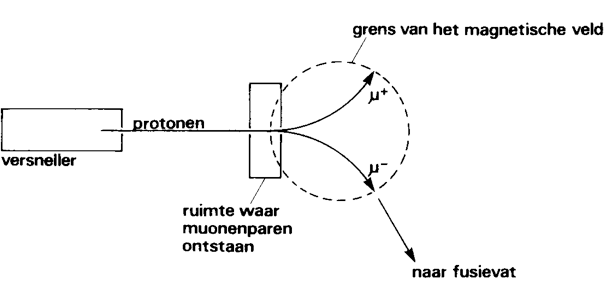
\includegraphics[scale=0.4]{versnellen_B-veld}
    \caption{De protonen worden worden versneld. Door botsingen met deze protonen 
    ontstaan muonen die op hun beurt in een magneetveld door hun lading gesplitst 
    worden in twee bundels.}
    \label{fig:versnellen_B-veld}
\end{figure}


\question
 Leg uit welke richting het magnetische veld in \ref{fig:versnellen_B-veld} heeft.
\makelines{2} 
 
\begin{solution} 
\end{solution} 



 In de grondtoestand van een waterstofatoom wordt de gemiddelde afstand r 
 tussen de atoomkern en het negatieve deeltje gegeven door: 
\begin{equation}
    r = c \cdot \frac{ (m_k + m)}{(m_k \cdot m)}
\end{equation}

Hierin is c een constante, m de massa van het negatieve deeltje en mk de 
massa van de atoomkern. In het tritiumatoom ($^3_1H$) in de grondtoestand bevindt 
het elektron zich op $\SI{5,3e-11}{\meter}$ van de atoomkern.
Als een negatief muon in de omgeving van een tritiumatoom komt, verdringt 
dit het elektron.

\question
Bereken de afstand van het muon tot de tritiumkern in de grondtoestand van dit `muonic hydrogen'.
\makelines{3} 
\begin{solution} 
 
\end{solution} 


Indien dit `muonic hydrogen' een waterstofmolecuul nadert dat bestaat uit een
deuteriumatoom en een tritiumatoom (respectievelijk $^2_1H$ en $^3_1H$), komen de
kernen van het `muonic hydrogen' en het deuteriumatoom voldoende dicht bij elkaar
te liggen om met elkaar te reageren tot helium en een neutron. De
heliumkern en het neutron vliegen weg, terwijl het muon achterblijft.
Het muon is nu beschikbaar om een nieuwe fusiereactie te veroorzaken.
Het onderzoek naar koude kernfusie is er op gericht, te bereiken dat één
muon vele kernfusies veroorzaakt voordat het vervalt.

\question 

Bereken hoeveel van deze kernreacties minstens nodig zijn om de energie 
terug te winnen die nodig is voor de creatie van één muonenpaar.
\makelines{3} 
\begin{solution} 
 
\end{solution} 

\section{Muonic Hydrogen}

Het muon is een deeltje wat lijkt op het elektron maar is zwaarder. 
In `muonic hydrogen' is het muon gebonden aan het atoom op de plek waar zich normaal het elektron bevindt.
`Muonic hydrogen' is in dit geval een gebonden toestand van een proton en een muon. 
In veel leerboeken en Binas kun je vinden dat de ionisatie energie van waterstof $\SI{-13,6}{\kilo\\electronvolt}$ is.
\question
Zoek in Binas de eigenschappen van het muon op.
\makelines{3}

\question
Zoek in Binas de formule voor elektrische kracht op.
\makelines{2}

\begin{solution} 
 
\end{solution} 

De elektrische kracht zorg ervoor dat het muon in een baan rond de kern blijft bewegen.
Zie \ref{fig:Muon_waterstofatoom}.
Deze kracht zorgt voor de `cirkelversnelling', die nodig is om in de baan te blijven.

\begin{eqnarray*}



\begin{figure}[h]
\centering
\begin{tikzpicture}
\draw [thick] (0, 0) circle (0.6 cm) node {\huge+};
%\draw [dashed] (0,0) circle (4 cm);
\draw [thick] (85:4cm) circle (.4 cm) node {$\mu^-$};
\draw [dashed,thick] (95:4cm) arc (95:435:4cm); 
\draw[thick,->] (0,0) -- (85:1.6cm) node [right] {$\vec{F}_{p, \mu}$};
\draw[thick,->] (85:4 cm) -- (85:2.4cm) node [left]{$\vec{F}_{\mu,p}$};
\end{tikzpicture}
\caption{Muon waterstofatoom}
\label{fig:Muon_waterstofatoom}
\end{figure}

\begin{figure}
\centering
\foreach \n in{6}{%
\begin{tikzpicture}
 \begin{axis}[axis equal,
    xmin=-3,xmax=3,
    ymin=-3,ymax=3,
    axis lines=none]
 \addplot[samples=400,domain=0:2*pi,thick] ({(2+.3*cos(deg(\n*x)))*cos(deg(x))},{(2+.3*cos(deg(\n*x)))*sin(deg(x))});
 \addplot[samples=40,domain=0:2*pi,dashed] ({2*cos(deg(x))},{2*sin(deg(x))});
 \node at (axis cs:0,0){$n=\n$};
\end{axis}
\end{tikzpicture}
}
\caption{in dit figuur zien we een patroon van een staande golf over de baan van
het muon. Het staande golf patroon moet `precies' passen op de omtrek van de baan.}
\label{fig:golven_waterstofatoom}
\end{figure}



\end{questions} 
\end{document}
